\chapter{Introdução}
\label{cap:introducao}

Esse capítulo apresenta de maneira geral aspectos e características da plataforma
ElixirBench. Abordaremos aspectos técnicos, como linguagem, licença, funcionalidades
e também aspectos não técnicos, como história, utilização e outros.

O projeto ElixirBench, escolhido para a disciplina, é uma ferramenta
de integração contínua, como Travis ou GitlabCI, porém destinada para a execução
de testes de desempenho (\textit{benchmarks}) e disponível apenas para projetos escritos na
linguagem de programação Elixir. A ideia geral é ter a execução dos testes
de desempenho a cada nova mudança ou nova versão lançada. Desta forma, o
papel da ferramenta é executar os testes de um repositório a partir de um monitoramento
automático das suas mudanças, coletando e disponibilizando métricas de desempenho,
como número de objetos alocados, iterações por segundo e outras. Ou seja, os
testes já existem em cada repositório, a ferramenta apenas os executa e disponibiliza
os resultados.

\section{Objetivos}

 O objetivo do projeto é oferecer aos desenvolvedores uma ferramenta que se integre
 facilmente ao repositório e também uma infraestrutura e recursos
 para monitoramento do desempenho de seus projetos. Aqueles que enxergam a questão
 do desempenho do código como um aspecto importante podem se beneficiar da mesma
 para prover soluções de maior qualidade. Algumas outras comunidades de linguanges
 de programação já possuem ferramentas semelhantes para medição e monitoramento do desempenho de bibliotecas.
 como o Speed\footnote{\url{https://speed.python.org}} do Python e RubyBench\footnote{\url{https://rubybench.org}} do Ruby.

\section{Histórico}

 O projeto nasceu em um evento de Hackathon chamado SpawnFest, em dezembro
 de 2017. A criação de três desenvolvedores foi \textbf{premiada como a melhor solução}.
 A descrição contida na página do evento\footnote{\url{https://spawnfest.github.io}} o descreve como:

 ``SpawnFest é...
 Uma competição anual de desenvolvimento online e aberta onde times de desenvolvedores
 ao redor do mundo tem exatamente um final de semana para criar a melhor aplicação
 sobre a BEAM que puderem.''
 \begin{center}
 (traduzido pelo autor)
 \end{center}

 Atualmente, o projeto encontra-se em desenvolvimento e não possui ainda uma versão em
 produção. Para atingir esta fase, tem recebido incentivos da comunidade
 Elixir para continuar evoluindo e ser colocado a uso. As atividades
 de desenvolvimento vieram principalmente das colaborações dos próprios criadores
 durante o Hackathon e tem seguido em ritmo menor com
 incentivos do programa Google Summer of Code 2018, que financia estudantes para contribuirem
 com softwares livres de organizações associadas. O projeto ElixirBench, 
 associado à organização BEAM Community\footnote{\url{https://summerofcode.withgoogle.com/organizations/6486585449644032}},
 está recebendo colaborações de um estudante, que no caso sou eu, e um
 mentor, criador da ferramenta.
 
\section{Principais Funcionalidades}

 O projeto funciona de maneira muito similar a uma ferramenta de integração
 contínua para execução de testes automatizados como TravisCI ou GitlabCI. Nessas
 ferramentas, por exemplo, os testes existem no repositório, escritos com alguma
 biblioteca de testes unitários, e a ferramenta de integração contínua apenas
 faz o download do projeto, instala suas dependências e executa estes testes
 para cada nova branch ou commit no repositório. Com isso é armazenado o histórico
 do resultado das execuções para cada branch, pull requests, etc, que pode
 ser visto em uma aplicação web.

 Atualmente as principais funcionalidades do projeto são:

 \begin{itemize}
   \item Disparar um \textit{job} de execução de testes manualmente para uma branch de um
   repositório desejado
   \item Execução de um \textit{jobs} isolados em containers Docker
   \item Permite instanciar múltiplos \textit{runners} isolados para execução de \textit{Jobs}
   \item Visualização simples dos resultados em uma página web
   \item Suporte a \textit{WebHooks} do Github para execução automática a cada novo
   evento de \textit{push} ou \textit{pull request} no repositório
 \end{itemize}

 O projeto ElixirBench, por sua vez, executa os testes escritos com a ferramenta
 Benchee, específica para coletar métricas de desempenho de códigos Elixir. Assim,
 os testes devem existir previamente no repositório, juntamente com o arquivo
 de configuração que define o ambiente adequado para execução dos testes, segundo
 as versões e dependências necessárias. O arquivo por sua vez deve ser colocado
 no diretório \textbf{benchee/config.yml}, buscado a partir da raiz do projeto.

\begin{figure}[!htb]
  \caption{Exemplo de arquivo de configuração \textbf{config.yml}}
  \centering
  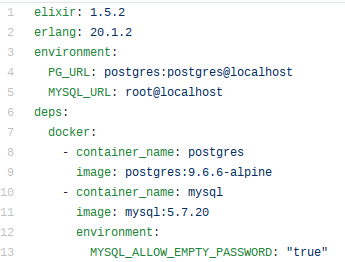
\includegraphics[width=82mm]{figuras/config-yml.png}
\end{figure}

A página web no entanto, ainda se encontra em um estágio inicial de desenvolvimento.
Uma ideia geral pode ser vista a seguir, que mostra a tela inicial com a listagem
dos repositórios mais populares e últimos \textit{jobs} executados.

\begin{figure}[!htb]
  \caption{Página inicial da ferramenta}
  \centering
  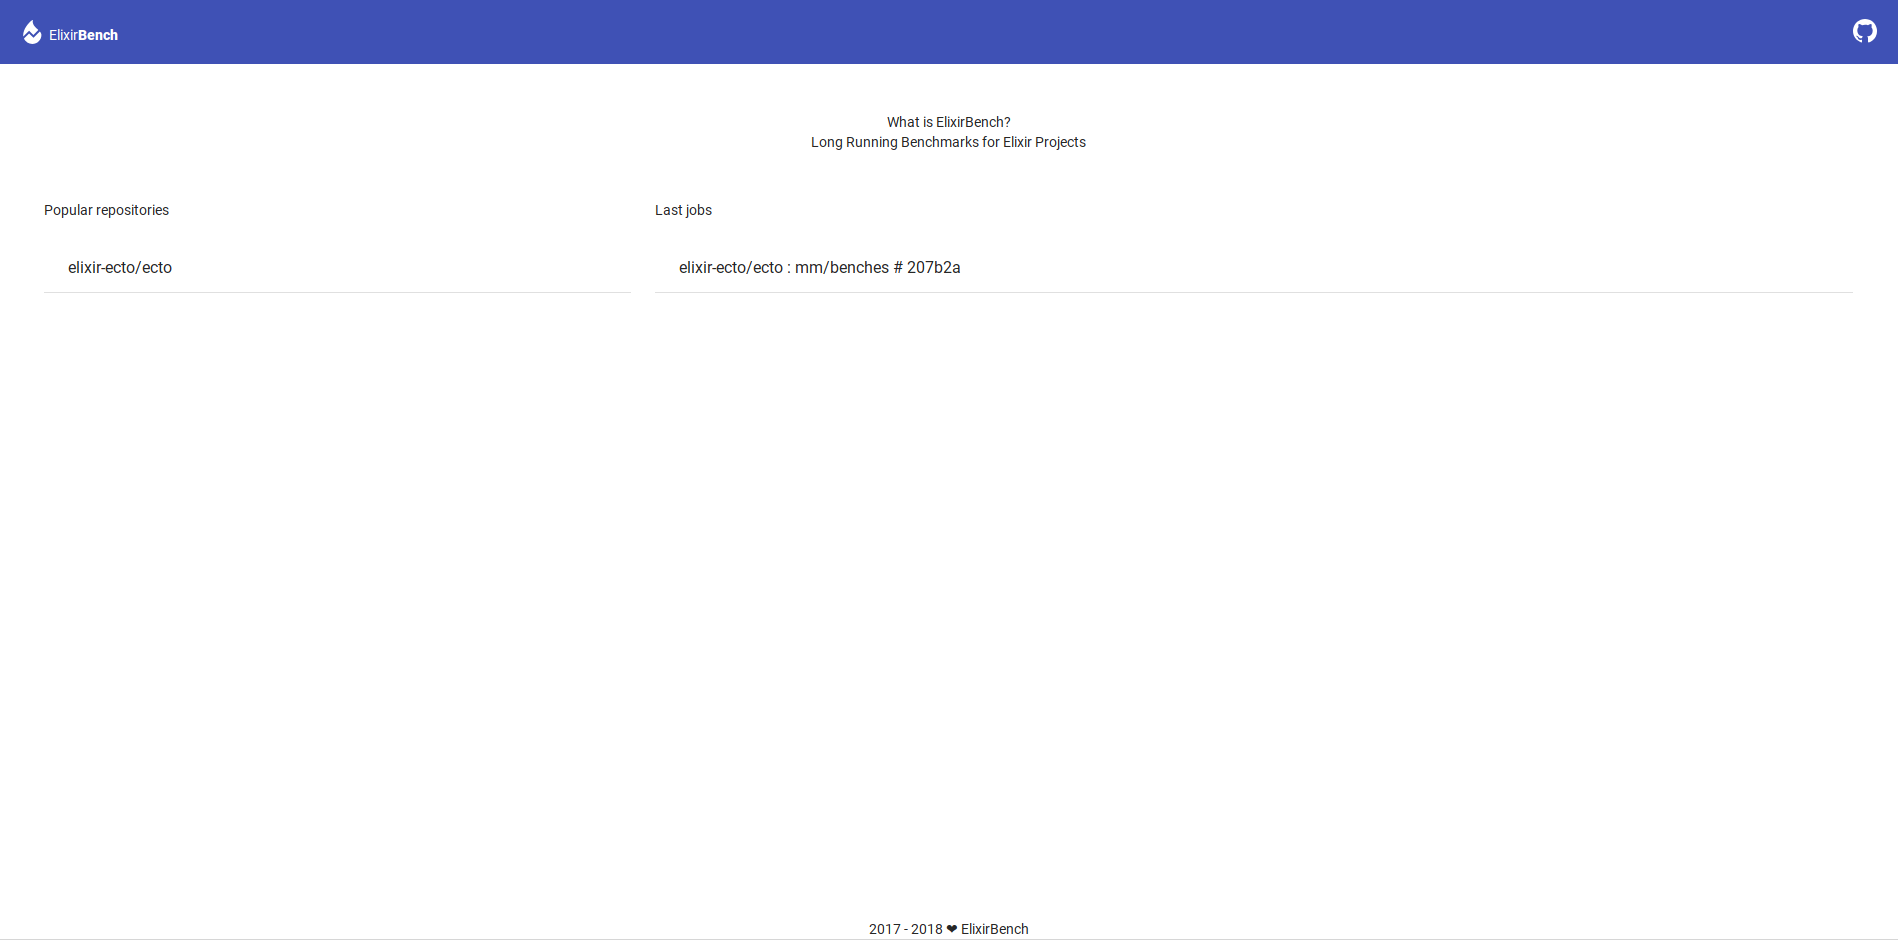
\includegraphics[width=\linewidth]{figuras/homepage.png}
\end{figure}

\section{Utilização ao redor do mundo}

 Como dito anteriormente, o projeto ainda não possui uma versão em produção que
 seja amplamente difundida. Os principais interessados até então, são desenvolvedores
 do projeto Ecto\footnote{\url{https://github.com/elixir-ecto/ecto}}, que será
 utilizado como prova de conceito e testes, sendo os primeiros utilizadores
 oficiais da ferramenta. Ecto é uma biblioteca que oferece uma linguagem específica
 de domínio em Elixir para escrita de \textit{queries} e interação com bancos de dados.

 A projeção do projeto, no entanto, é oferecer a todos os pacotes e projetos Elixir hospedados
 no GitHub um serviço para execução de testes de benchmarks, assim como faz a ferramenta
 TravisCI. Assim, mais de 6 mil pacotes cadastros no gerenciador de dependências
 Hex\footnote{\url{https://hex.pm}} poderão se beneficiar do projeto ElixirBench.
